\vspace*{4cm}
\begin{center}
\part{Point to Point Testinfrastruktur}\label{PointtoPointTestinfrastruktur}
\end{center}
\vspace*{\fill}
\clearpage

\section{P2P Konzept}\label{sec:P2PKonzept}

Im Nachfolgenden Abschnitt wird auf die Point to Point (P2P) Messung eingegangen. Ziel ist es die Verbindung auf MAC-Layer auszumessen und die aus Abschnitt ... aufgelisteten Messdaten zu erfassen. Dazu wird im folgenden auf das Messkonzept, den Messablauf und technische Einzelheiten eingegangen. 

\subsection{Anforderungen}\label{sec:AnforderungentP2P}

\todo[inline]{Anforderungen an P2P Software beschreiben}

\subsection{Konzept}\label{sec:KonzeptP2P}

Zur Realisierung der Point to Point Testinfrastruktur wurde auf eine \textit{One to Many} (1:n) Messprinzip gesetzt (auch als Broadcasting bekannt). Dies hat den Vorteil das mehrere Verbindungen gleichzeitig ausgemessen werden können. Der Nachteil dabei ist, dass die Messpfade nur unidirektional charakterisiert werden (nur von Master zu Slave oder Uplink-Pfad). Die Abweichung zwischen Up- und Downlink Pfad können durch wiederholen der Messung mit vertauschten Standorten verifiziert werden. 

\begin{figure} [H]
	\centering
	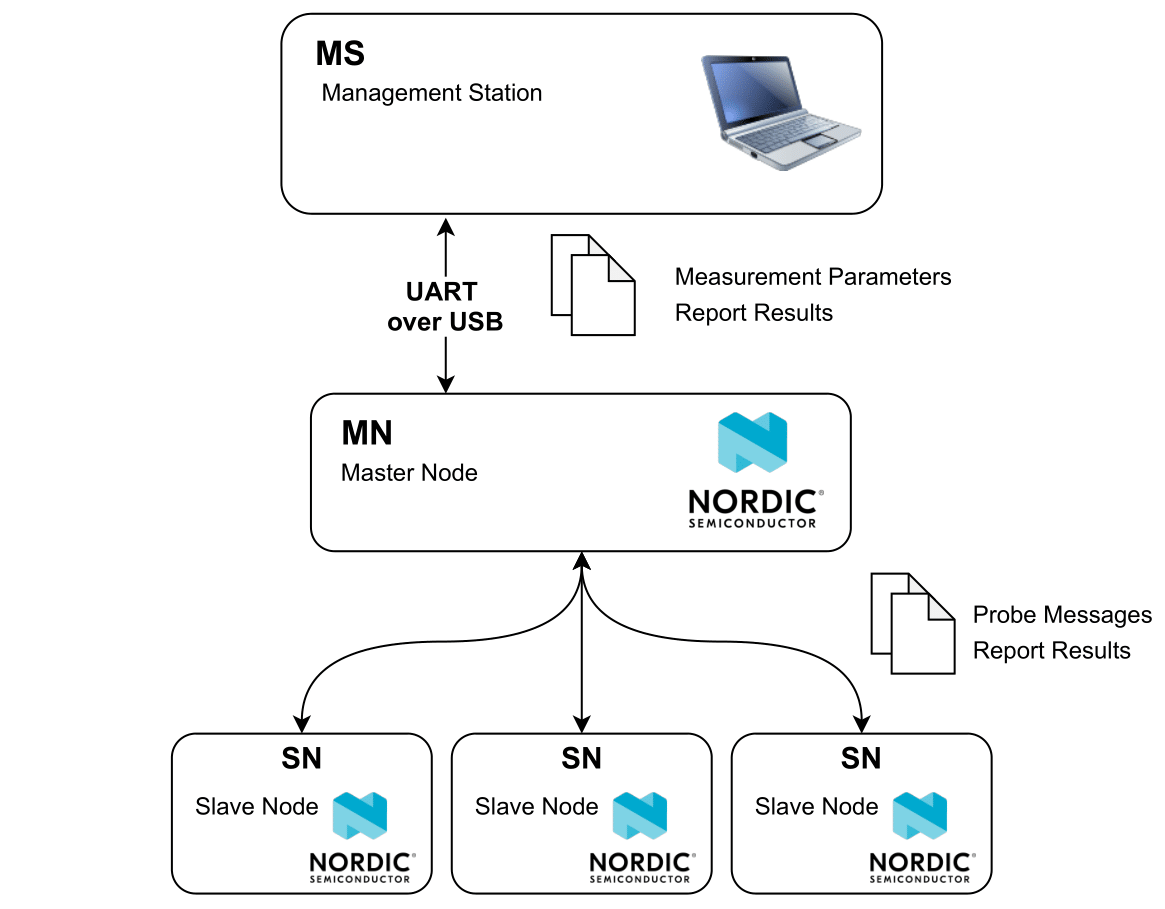
\includegraphics[width=0.8\textwidth]{Konzeptschema_P2P.png}
	\caption{Konzeptschema P2P Testinfrastruktur}
	\label{fig:KonzeptschemaP2P}
\end{figure}

Das in Abbildung \ref{fig:KonzeptschemaP2P} gezeigte Konzept besteht aus einer Managment Station, einem Master- und mehreren Slave Nodes. Über die Management Station können Messresultate angezeigt, sowie Messparameter eingestellt werden. Als Ausgangspunkt zur Messung dient der MN (Master Node). Er koordiniert den Messablauf und sendet \textit{Probe Packets} an alle SN (Slave Nodes). Diese Protokollieren die Anzahl empfangener \textit{Probe Packets} und melden ihre Messresultate an den MN zurück. Nach Empfang aller Resultate leitet der MN alle Messergebnisse an die MS weiter. Dort werden dem Benutzer die Messdaten dargestellt. Details zum Ablauf sind in Abschnitt \ref{sec:SoftundFirmware} aufgeführt. Eine mögliche Anwendung der Testinfrastruktur wird im folgenden Abschnitt \ref{sec:TestszenarienP2P} beschrieben.  

\subsection{Testszenarien}\label{sec:TestszenarienP2P}

Die P2P Testinfrastruktur ist als einfach zu bedienendes Tool konzipiert. Es kann eingesetzt werden um den Aufbau von PAN-Netzwerken zu optimieren. Mithilfe des Tools können zu Beispiel die Standorte der Teilnehmer eines Zigbee, Thread oder Bluetooth Mesh Netzwerks optimal gewählt werden. Zudem lassen sich während eines Messvorgangs gezielt Störungen in ein solches Netzwerk einbringen. Dadurch können die Netzwerke auf Störsicherheit geprüft werden. 

\todo[inline]{Testumgebungen sowie die Beziehungen der Knoten innerhalb der Point to Point Messung beschreiben.}

\subsection{Ablauf}\label{sec:AblaufP2P}
\todo[inline]{Ablauf eines Point to Point MAC Layer Benchmarks aus Anwendersicht beschreiben.}

\subsection{Messgrössen}\label{sec:MessgrössenP2P}
\todo[inline]{Erläuterung der Messgrössen die erfasst werden sollen. Inkl. Beschreibung wie dies technisch umgesetzt wird.}

\subsection{Messaufbau}\label{sec:Messaufbau}

\begin{figure} [H]
	\centering
	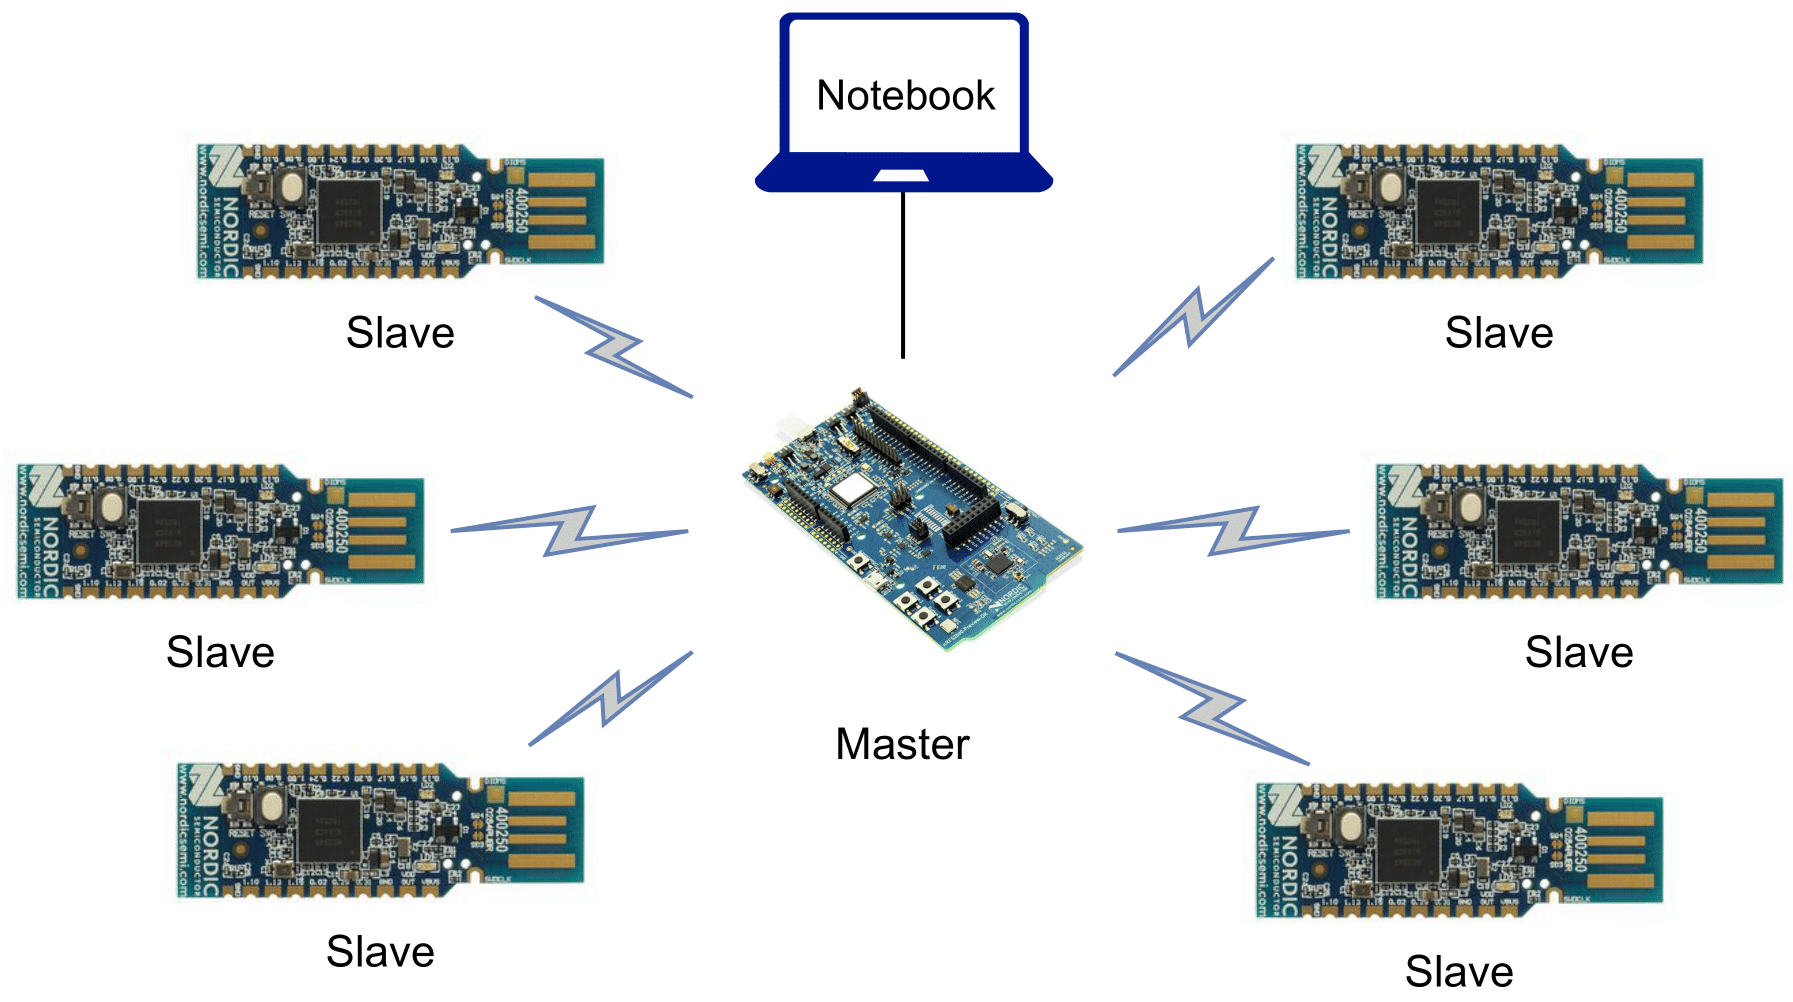
\includegraphics[width=0.8\textwidth]{Messaufbau_P2P.png}
	\caption{Messaufbau P2P Testinfrastruktur}
	\label{fig:MessaufbauP2P}
\end{figure}

\todo[inline]{Schema inkl. Beschreibung.}


\section{Bedienung Messinfrastruktur}\label{sec:BedienungMessinfrastruktur}


\subsection{Aufbau und Bedienung der Messinfrastruktur}\label{sec:AufbauundBedienungderMessinfrastruktur}
\todo[inline]{Bedienungsanleitung des Messaufbaus.}

\subsection{Interpretation der Messresultate für den Anwender}\label{sec:InterpretationderMessresultatefürdenAnwender}
\todo[inline]{Wie sind die Resultate zu interpretieren. Welche Schlüsse können/müssen aus den Resultaten gezogen werden. Welche Resultate bedeuten was?}


\section{Soft- und Firmware}\label{sec:P2PSoft-undFirmware}

\subsection{Soft- und Firmware}\label{sec:SoftundFirmware}

Die Software ist als zeit-diskrete Schrittkette aufgebaut. Jeder Schritt ist über ein fixes Zeitfenster definiert, wodurch der Ablauf rein zeitabhängig vorgegeben ist. Damit alle Teilnehmer synchron ihre Schrittketten abarbeiten, muss mithilfe einer Zeitsynchronisation auf den Master der exakte Startzeitpunkt kommuniziert werden. Unabhängig vom Zustand des aktiven Schrittes, darf dieser sein Zeitfenster nicht überschreiten, ansonsten fällt die Schrittkette ausser Takt. 

\begin{figure} [H]
	\centering
	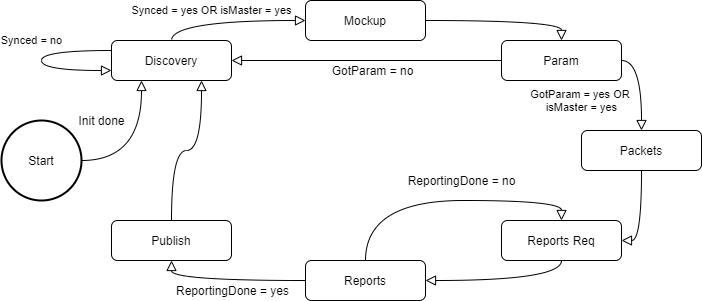
\includegraphics[width=1.0\textwidth]{Software_Flowgraph_P2P.png}
	\caption{Schrittkette P2P Testinfrastruktur}
	\label{fig:FlowgraphP2P}
\end{figure}

Abbildung \ref{fig:FlowgraphP2P} zeigt die Schrittkette für den Master, sowie für die Slave-Nodes. Der Ablauf zeigt die Schritte, sowie die Bedingungen der Transitionen zwischen den Schritten. Jedoch muss beachtet werden das jeder Schritt immer eine bestimmte Zeit aktiv bleibt. Somit ist ersichtlich das der \textit{Packets-State} nach Ablauf seines Zeitfensters immer zum \textit{ReportsReq-State} führt. Wobei der Wechsel nach dem \textit{Discovery-State} von verschiedenen Bedingungen abhängig ist. \\

Die Funktion der Schritte wird im Folgenden grob beschrieben. Zur genauen Untersuchung ist der Source Code unter \cite{github_p6_software_p2p_2020} verfügbar.  \\

\begin{itemize}
	\item \textbf{\textit{Discovery:}} Der Master verteilt die Zeitsynchronisation an die Slaves. Die Slaves synchronisieren sich auf das Signal des Masters auf, sofern sie in seiner Reichweite liegen. Hat ein Slave sich nicht Synchronisieren können verweilt dieser im \textit{Discovery-State}. Der Master darf immer zum nächsten Schritt voranschreiten. 
	\item \textbf{\textit{Mockup:}} Der Master wartet auf eine Antwort der einzelnen Slaves. Jeder Slave generiert einen zufälligen Timeslot um sich beim Master anzumelden. Der Master führt alle Slaves, welche sich gemeldet haben in einer Liste auf. Ist diese Liste leer (hat sich kein Slave gemeldet), so wird der Master zum \textit{Discovery State} zurückkehren. Ist ein Slave bereits beim Master angemeldet, so muss sich dieser nicht erneut anmelden. 
	\item \textbf{\textit{Param:}} Der Master versendet die Packets-Parameter (Mode, StartChannel, StopChannel, etc) auf welchen er die Probe-Packets versendet. Erhält ein Slave keine Daten so kehrt er in den \textit{Discovery-State} zurück. 
	\item \textbf{\textit{Packets:}} Der Master versendet \textit{Probe Packets} auf den zuvor Kommunizierten Einstellungen. Die Slaves empfangen diese Daten und zählen die Anzahl erfolgreich empfangener Pakete und erfassen weitere Messdaten. 
	\item  \textbf{\textit{Reports Req:}} Nach dem ausmessen beginnt der Master mit dem einsammeln der einzelnen Slave Reports. Dazu sendet er an jeden Slave in seiner Liste (aus dem \textit{Mockup-State}) Report-Anfragen, sogenannte \textit{Reports-Requests}. Die Slaves warten auf einen \textit{Report Request} vom Master. 
	\item  \textbf{\textit{Reports:}} Der Slave, welcher den Request bekommen hat, sendet seinen Report zum Master. Dies muss innerhalb einer gewissen Zeit erfolgen. Sendet ein Slave nach einer gewissen Anzahl von Versuchen keine Reports, wo wird er aus der Liste der gemeldeten Slaves entfernt. Sobald der Master alle Reports von allen Slaves empfangen hat, meldet er über eine spezielle \textit{Reports-Request-Message} an alle Slaves, dass das Reporting beendet ist.
	\item  \textbf{\textit{Publish:}} Im \textit{Publishing-State} hat der Master Zeit die Daten an die Übergeordnete stelle zu Übermitteln (USB-UART). Die Slaves können in diesem State Energie Sparen. Alle Teilnehmer beginnen wieder im \textit{Discovery-State}, wo sie sich neu Synchronisieren. 
\end{itemize}





\todo[inline]{Beschreibung der Node-Firmware sowie der Auswertesoftware auf dem Raspi.}

\subsection{Low Level Radio Driver}\label{sec:LowLevelRadioDriver}

Die Kommunikation über das Radio-Interface wurde mittels einem eigens entwickeltem Radio-Driver, speziell für die nRF52 / nRF53 SOCs ermöglicht. Dieser stellt die nötigen Funktionen für die P2P Testinfrastruktur zur Verfügung. Zum Beispiel kann die Mode- und Kanalwahl sowie das Senden und Empfangen von Daten mittels simplen Kommandos erfolgen. Zur Entwicklung diente das \textit{Radio Test Example} \cite{nrf_connect_sdk_radio_test_example_2020} als Vorlage. Der Radio-Driver steuert mithilfe der \textit{NRF-HAL Radio Library} oder über direkten Zugriff auf die Peripherie-Register das Radio-Interface an.

\begin{figure} [H]
	\centering
	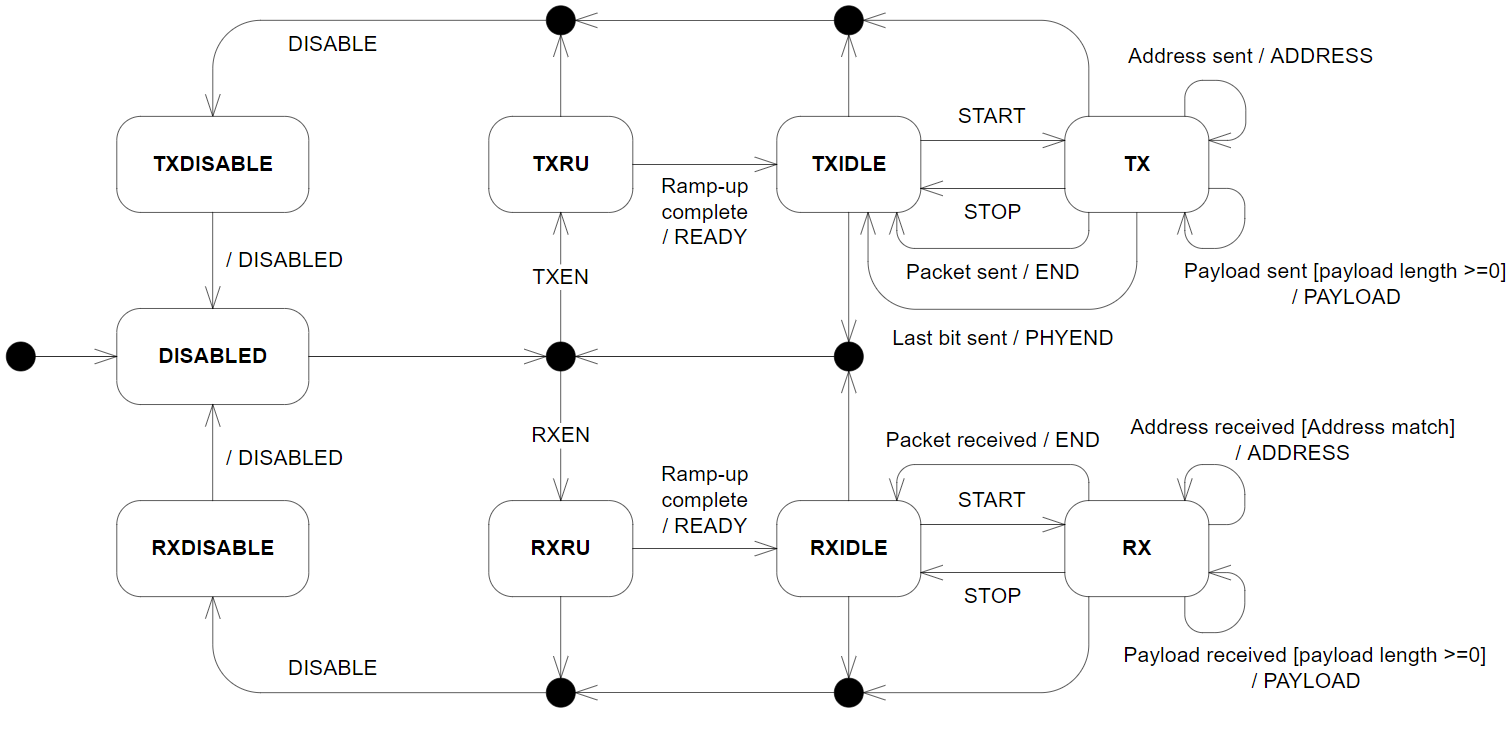
\includegraphics[width=1.0\textwidth]{nRF52840_Radio_states.png}
	\caption{Radio States \cite{nordic_semi_nrf_infocenter_radio_states_2020}}
	\label{fig:RadioStatesP2P}
\end{figure}

Die Radio Hardware der nRF52 und nRF53 SOCs verfügt über verschiedene Zustände (siehe Abbildung \ref{fig:RadioStatesP2P}). Abhängig von der gewünschten Operation (Senden oder Empfangen), werden die States abgearbeitet. Um Energie zu sparen wird nach Abschluss der gewünschten Tätigkeit immer in den Disabled-State gewechselt. Zusätzlich erfolgt das Benachrichtigen des Radio Drivers von der Hardware mittels Interrupts, wodurch der Energieverbrauch zusätzlich minimiert wird.

\begin{figure} [H]
	\centering
	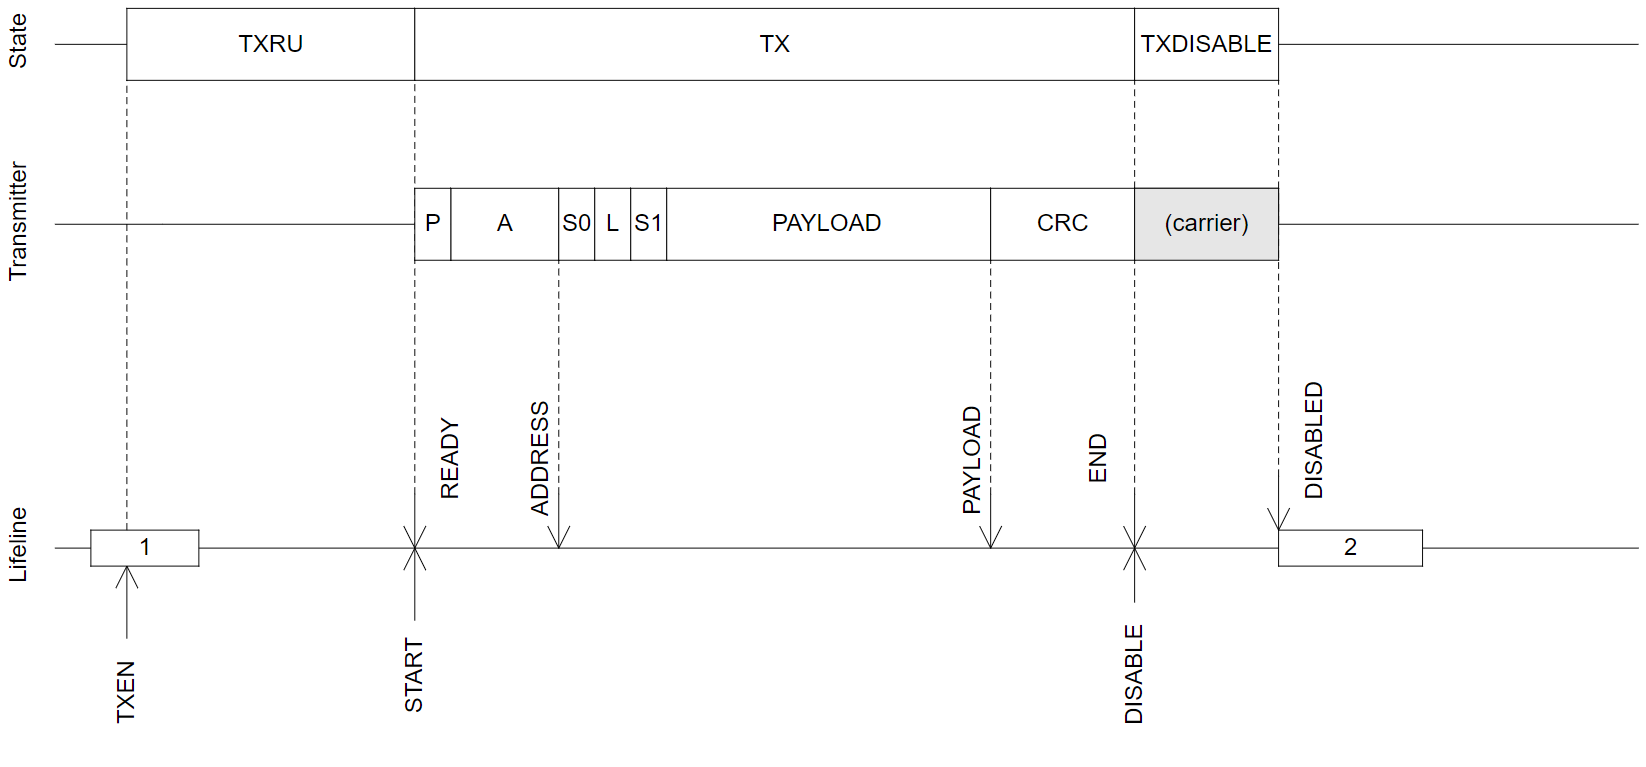
\includegraphics[width=1.0\textwidth]{nRF52840_Radio_Transmit_Sequence_with_Shorts.png}
	\caption{Sende-Ablauf mit Verknüpfungen \cite{nordic_semi_nrf_infocenter_radio_transmit_sequence_2020}}
	\label{fig:RadioTransmitSequP2P}
\end{figure}

Abbildung \ref{fig:RadioTransmitSequP2P} zeigt den Ablauf beim Senden eines Pakets. Die zu sendenden Daten (Payload) müssen vorgängig im RAM vorliegen. Anschliessend wird der Packet Pointer des Radio-Interface auf die entsprechende Speicher-Adresse eingestellt. Zu beachten gilt es das im ersten Byte die Länge der Payload angegeben sein muss. Diese wird vom Radio Driver automatisch ergänzt. Zusätzlich kann ein Adress-Feld den Sende-Daten mitgegeben werden. Nach dem vollständigen Konfigurieren des Radio-Interface wird das Senden durch den Befehl TXEN initiiert. Mithilfe von Verknüpfungen (Shorts) wird nach dem Ready-Event automatisch der Start-Task ausgelöst. Das Senden läuft also nach dem Initiieren vollautomatisch ab. Der Radio-Driver wartet lediglich auf das auslösen des Disabled-Events. Das Senden ist erfolgreich abgeschlossen und der Funktionsaufruf kehrt zum Hauptprogramm zurück. Das Senden mittels CCA wird im \textit{IEEE802.15.4-Mode} unterstützt. Dazu wird vor dem Senden der Kanal abgehört um Kollisionen zu vermeiden. Mittels dem RXEN Befehl wird der CCAStart-Task aktiv. Dieser führt abhängig vom Konfigurierten CCA-Modus eine Prüfung des Kanals durch. Ist der Kanal nicht belegt wird ein CCAIdle-Event generiert, welcher mittels Verknüpfung automatisch den TXEN-Task Startet (siehe Abbildung \ref{fig:CCAIDLEP2P}). Sendet ein andere Teilnehmer momentan auf dem Kanal wird ein CCABusy-Event generiert, welcher ebenfalls den Disable-Taks ausführt (siehe Abbildung \ref{fig:CCABUSYP2P}). Somit Enden beide Varianten (Idle und Busy) im Disabled-State, wobei beim einen keine Daten gesendet werden konnten. \cite{nordic_semi_nrf_infocenter_radio_transmit_sequence_2020}

\begin{figure}[!htbp]
	\begin{minipage}{0.49\textwidth}
		\centering
		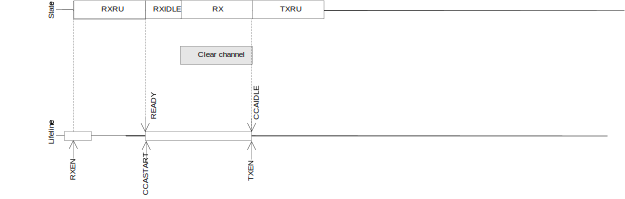
\includegraphics[width=\textwidth]{cca.png}
		\caption[Sende-Ablauf mit CCA Idle]{CCA Prüfung (Idle Event) \cite{nordic_semi_nrf_infocenter_radio_ieee_operation_2020}}
		\label{fig:CCAIDLEP2P}
	\end{minipage}
	\begin{minipage}{0.49\textwidth}
		\centering
		\includegraphics[width=\textwidth]{cca_busy.png}
		\caption[Sende-Ablauf mit CCA Busy]{CCA Prüfung (Busy Event) \cite{nordic_semi_nrf_infocenter_radio_ieee_operation_2020}}
		\label{fig:CCABUSYP2P}
	\end{minipage}
\end{figure}

\begin{figure} [H]
	\centering
	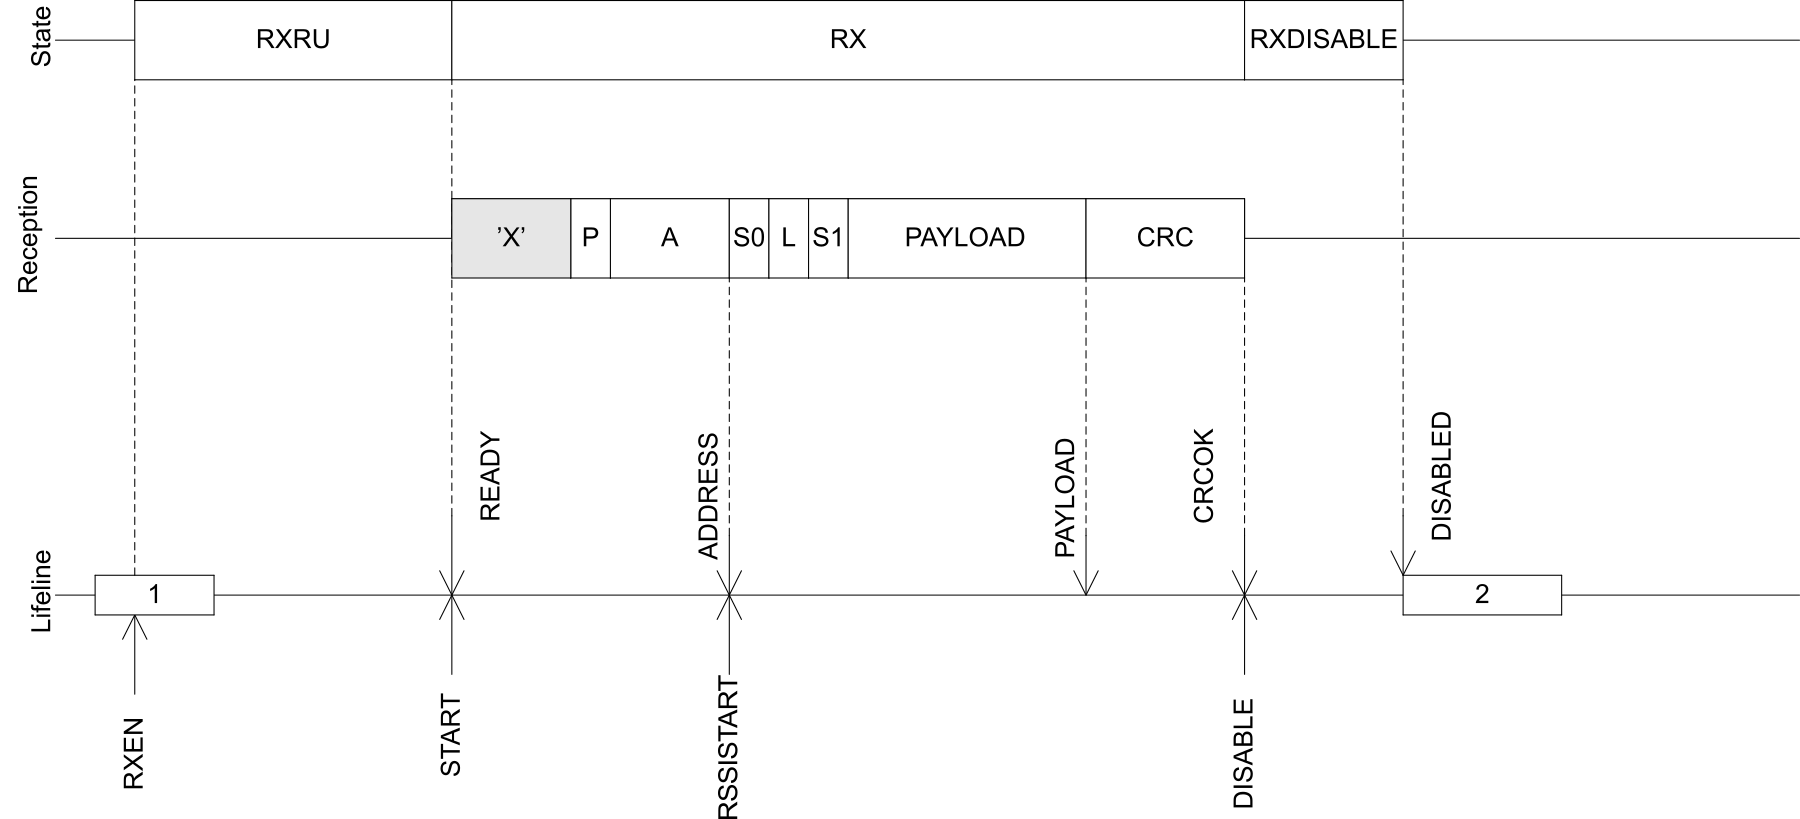
\includegraphics[width=1.0\textwidth]{nRF52840_Radio_Receive_Sequence_with_Shorts.png}
	\caption{Empfangs-Ablauf mit Verknüpfungen \cite{nordic_semi_nrf_infocenter_radio_receive_sequence_2020}}
	\label{fig:RadioReceiveSequP2P}
\end{figure}

\todo[inline]{Bild mit RSSI Start ergänzen}

Der Ablauf zum Empfangen eines Pakets wird in Abbildung \ref{fig:RadioReceiveSequP2P} dargestellt. Grundsätzlich ist der Ablauf gleich Aufgebaut wie beim Senden von einem Paket. Nach Initiieren mittels dem RXEN-Befehl fährt der Empfänger hoch und wartet auf den Empfang eines Pakets. Nach eingehen einer Preamble-Sequenz wird das Address-Feld geprüft. Dieses kann vorgängig festgelegt werden um nur Pakete mit übereinstimmender Adresse zu empfangen. Bei allen BLE-Modes erfolgt die Prüfung auf Hardware-Ebene (ohne Interaktion der CPU) ab. Beim \textit{IEEE802.15.4-Mode} steht dieses Feature nicht zur Verfügung. Das vergleichen des Adress-Feldes muss der Radio-Driver selbst übernehmen. Um die Signalstärke (RSSI) vom eingehenden Paket zu messen, wird eine Verknüpfung zwischen dem \textit{Address-Event} und dem \textit{RSSIStart-Task} aktiviert. Nach erfolgreichem Prüfen der CRC Checksumme wird mittels einer Verknüpfung des CRCOK-Event der Disable-Task ausgeführt. Beim Empfangen eines Pakets wartet der Radio-Driver während eines gewissen Timeouts auf den Disabled-Event. Die Empfangsfunktion gibt die Restzeit des Timeouts in Millisekunden zurück, wodurch sich ein erfolgreiches Empfangen prüfen lässt. Das Bufferhandling übernimmt der Radio-Driver und erwartet beim Senden und Empfangen von Daten eine vordefinierte \textit{Radio-Packet-Structure}. Zu beachten gilt es das die Daten erst nach dem End-Event  vollständig abgearbeitet wurden, da der Zugriff von der Hardware über DMA erfolgt. Ebenfalls wurde festgestellt das beim wechseln auf oder von dem \textit{IEEE802.15.4-Mode} der Kanalwechsel vor dem Modewechsel erfolgen muss. Ansonsten werden keine Pakete empfangen. \cite{nordic_semi_nrf_infocenter_radio_receive_sequence_2020}


\subsection{Broadcasting Collisions Probability}\label{sec:BroadcastingCollissionsProbability}

Kollisionen entstehen wenn mehrere Teilnehmer gleichzeitig auf dem selben Kanal (Frequenz) senden. Dabei stören sich die beiden Sender und es kann sein das der Empfänger keine Daten empfangen kann. Dies ist leider nicht immer zu vermeiden, zum Beispiel wenn sich mehrere Teilnehmer neu mit dem Netz verbinden möchten. Im Fall der P2P-Testinfrastruktur entsteht ein solcher Fall im Mockup-State. Hier soll sich jeder Slave, welcher dem Master noch unbekannt ist, auf die Discovery-Anfrage des Masters melden. Die Lösung ist das jeder Slave einen zufälligen Zeitpunkt zum Antworten auswählt. Doch wie lange muss das Zeitfenster sein in welchem ein Slave einen Zeitpunkt zufällig auswählen darf? \\

Angenommen es gibt $N$ Teilnehmer, welche $t_a$ Sekunden brauchen um eine Antwort zu Senden. Zusätzlich existieren $N_{ch}$ verschiedene Kanäle auf welchen die Teilnehmer antworten können. Die Wahrscheinlichkeit das sich zwei Sender nicht überlappen $P_{miss}$ im Zeitfenster $t_I$ Sekunden lässt sich gemäss Formel \ref{eq:BroadcastingMissProbability} bestimmen. \cite{rk_how_to_deal_with_broadcasting_collision_2020}

\begin{equation}\label{eq:BroadcastingMissProbability}
P_{miss} = (1- \frac{2 \cdot t_a}{N_{ch}} \cdot t_I)^{N-1}
\end{equation}

Die folgenden Werte wurden zur Berechnung des Zeitfensters im Mockup-State verwendet:

\begin{itemize}
	\item $N = 50$
	\item $t_a = 5ms$
	\item $N_{ch} = 3$
	\item $t_I = 1.2s$	
\end{itemize} 

Somit liegt die Wahrscheinlichkeit das alle 50 Nodes sich verfehlen bei 85\%. 

\subsection{Zeitsynchronisation}\label{sec:ZeitsynchronisationP2P}

Die Zeitsynchronisation wurde mittels einer Offset Kompensation gelöst. Der Zeitgeber (Master) sendet seine Zeit (Timestamp) über einen Broadcast an alle Teilnehmer in der Umgebung. Die Slaves vergleichen den empfangene Master-Zeit mit ihrer lokalen Zeit und errechnen den Unterschied (Offset) zwischen dem Master-Timestamp und Slave-Timestamp. Somit können sie ihre Zeit mittels an die des Masters angleichen. Das Prinzip ist realtiv simpel birgt jedoch einige Ungenauigkeiten. Die Verzögerungszeit zwischen dem auslesen des Master-Timestamp bis zum empfangen und vergleichen mit dem Slave-Timestamp ist sehr relevant.  

\begin{figure} [H]
	\centering
	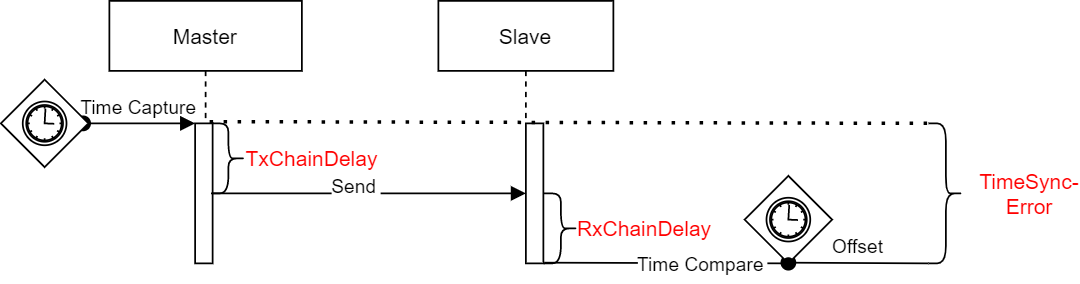
\includegraphics[width=1.0\textwidth]{Timesync_Basic.png}
	\caption{Zeitsynchronisation über Offset mit Fehler}
	\label{fig:TimesyncBasicwithErrorP2P}
\end{figure}

Wie in Abbildung \ref{fig:TimesyncBasicwithErrorP2P} ersichtlich entsteht beim Auslesen der Zeit bis zum Senden eine Verzögerung die TxChainDelay, sowie beim Empfänger die RxChainDelay. Da Ziel ist es diese Verzögerungen so gering wie möglich zu halten. 

\begin{figure} [H]
	\centering
	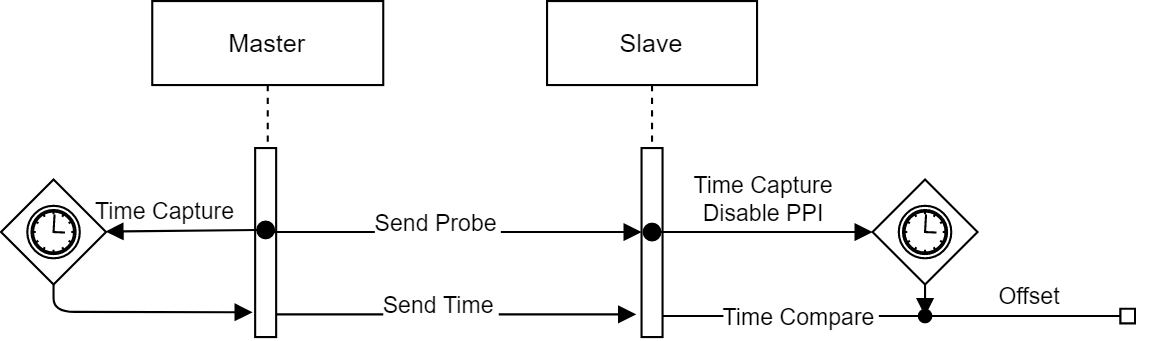
\includegraphics[width=1.0\textwidth]{Tiesync_Advanced.png}
	\caption{Zeitsynchronisation über Offset mit PPI}
	\label{fig:TimesyncwithPPIP2P}
\end{figure}

Die Lösung wird in Abbildung \ref{fig:TimesyncwithPPIP2P} gezeigt. Der nRF52840 SOC verfügt über ein PPI (Programmable peripheral interconnect). Mithilfe des PPI lassen sich verschiedene Events und Tasks direkt Verknüpfen, ohne das die CPU dabei involviert ist. Dies führt zu minimalen Verzögerung (ca. 1/16 us) zwischen Event und Task. Dazu wird der Event, dass ein Packet erfolgreich Gesendet wurde (Radio-End-Event), mit dem Task zum Erfassen des Synctimers (Synctimer-Capture-Task) verknüpft. Beim Slave wird der Event, dass ein Packet erfolgreich Empfangen wurde (Radio-CRCOK-Event), mit dem Task zum Erfassen des Synctimers (Synctimer-Capture-Task) verknüpft. Nach dem empfangen muss der Slave diesen PPI sofort deaktivieren, da ein direkt folgendes Paket ebenfalls ein Erfassen des Timers auslöst. Der Master wird nach deaktivieren des PPI mit einem Folge-Paket seine Master-Zeit dem Slave mitteilen, welche zum Zeitpunkt des Probe-Packets registriert wurde. Der Slave errechnet den Offset gemäss Formel \ref{eq:TimesyncOffsetSynctimeCalc} und die Synchronisierte-Zeit mit der Formel \ref{eq:TimesyncSynctimeCalc}. \cite{nordic_semi_nrf_infocenter_ppi_2020}

\begin{equation}\label{eq:TimesyncOffsetSynctimeCalc}
T_{Offset} =  T_{Master} - T_{Slave} 
\end{equation}

\begin{equation}\label{eq:TimesyncSynctimeCalc}
T_{Sync} =  T_{Slave} + T_{Offset} 
\end{equation}

Zur Verifikation der Zeitsynchronisation wurde ein Oszilloskop an jeweils einen GPIO-Pin am Master und einen am Slave angeschlossen. Auf dem Master und Slave wurden nacheinander Timer-Interrupts registriert, welche relativ zur synchronisierten Zeit auf dem Master und Slave genau gleichzeitig auslösen. Mithilfe eines PPI-Kanals wurde der Interrupt-Event auf den GPIO-Pin Verknüpft. Beim auslösen des Interrupts wird der Zustand des GPIO-Pins getoggelt. Somit wird die Abweichung Präzise auf dem Oszilloskop ersichtlich.

\begin{figure} [H]
	\centering
	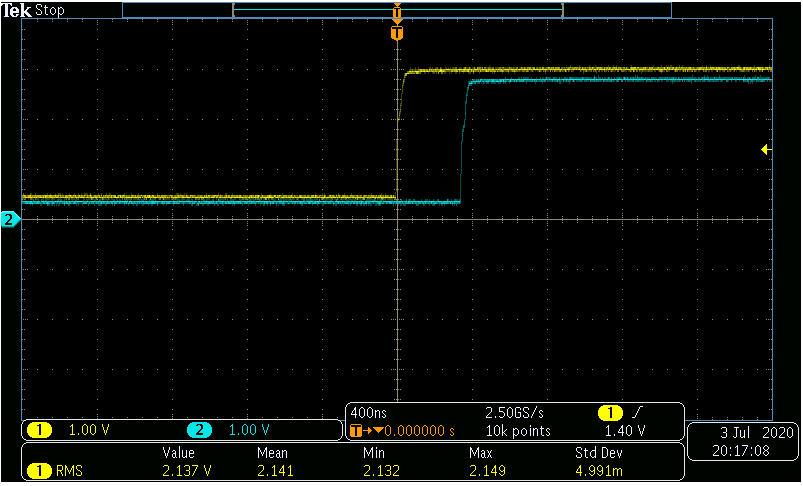
\includegraphics[width=1.0\textwidth]{Messungen Timesync (100ns 1200ns).png}
	\caption{Verifikation Zeitsynchronisation}
	\label{fig:TimesyncVerifikationP2P}
\end{figure}

Abbildung \ref{fig:TimesyncVerifikationP2P} zeigt den Signalverlauf der GPIOs vom Master (gelb) und Slave (blau). Anfänglich lagen die Abweichungen im Bereich von ca. 40us. Durch Wiederholungen der Messung konnte dieser Fehler als systematisch identifiziert werden. Mithilfe einer Korrektur um 40us konnte die Genauigkeit in den Bereich von 100ns bis 1200ns reduziert werden. Eine Abweichung der Zeitsynchronisation von ca. 1us sollte genügend genau sein um als gute Grundlage für die Statemachine aus Abschnitt \ref{sec:SoftundFirmware} zu dienen. 
 

\todo[inline]{Wie wurde die Zeitsynchronisation umgesetzt? Wie relevant ist diese für die Messungen?}